\graphicspath{{./fifth/img/}} % path to graphics

\section*{\LARGE Введение}
\addcontentsline{toc}{section}{Введение}
Давайте создадим модель небольшого аэропорта с двумя гейтами. Пассажиры
будут прибывать в аэропорт и регистрироваться на рейс (если они не сделали
этого заблаговременно через интернет). Затем все пассажиры должны будут
пройти процедуру предполетного досмотра, после чего они смогут направиться
в зону ожидания перед гейтами, дожидаясь начала посадки на свой рейс. При
объявлении начала посадки, пассажиры направляются к соответствующему
гейту. У гейта служащие аэропорта проводят проверку посадочных талонов,
после чего пассажиры проходят на посадку на самолет.\par
Процесс создания модели будет разбит на шесть фаз. В последней из них вы
научитесь считывать данные из базы данных (мы считаем информацию о
совершаемых рейсах из файла Microsoft Excel).

\clearpage

\section*{\LARGE Выполнение практической работы}
\addcontentsline{toc}{section}{Выполнение практической работы}

\section{Задание потока пешеходов}
Мы начнем с создания простой модели, в которой пассажиры прибывают в
аэропорт и движутся к выходу на посадку. Логику модели мы зададим с
помощью блоков \textit{Пешеходной библиотеки AnyLogic}.\par
Обычно создание пешеходных моделей начинается с добавления плана
моделируемого пространства и рисования стен, обозначенных на плане.\par
Теперь давайте зададим стены, ограничивающие моделируемое пространство.
Для этого мы воспользуемся специальными элементами разметки пространства,
созданными для пешеходного моделирования в AnyLogic. Все эти фигуры можно
найти в палитре Пешеходная библиотека, в разделе Разметка пространства.\par
Обычно создание модели начинается с рисования стен поверх имеющегося
плана моделируемого помещения. Стены в пешеходном моделировании
представляют собой объекты, через которые пешеходы не могут пройти.\par
Мы нарисовали ключевые объекты моделируемого пространства с помощью
фигур разметки пространства. Теперь можно приступить к заданию логики
модели с помощью блоков Пешеходной библиотеки.\par
Ваша диаграмма процесса должна выглядеть так, как
на рисунке~\ref{{fig:model:easy}}.

\begin{image}
	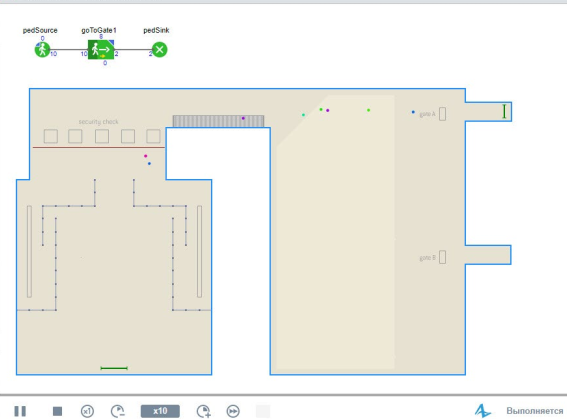
\includegraphics[width=0.9\textwidth]{Screenshot from 2023-04-11 14-47-00}
	\caption{Движение пешеходов в простой модели}
	\label{fig:model:easy}
\end{image}

\section{Создание 3D анимации}
Теперь давайте добавим в нашу модель 3D анимацию. Для этого, как мы уже
знаем, нам понадобится добавить 3D окно, камеру и 3D изображение
пассажира. Начнем именно с задания трехмерной фигуры анимации, что
потребует создания нового \textbf{Типа пешехода}.\par
Запустив модель увидим, что 3D анимация отображается
с учетом заданного расположения камеры (Рисунок~\ref{fig:3d:anim}).

\begin{image}
	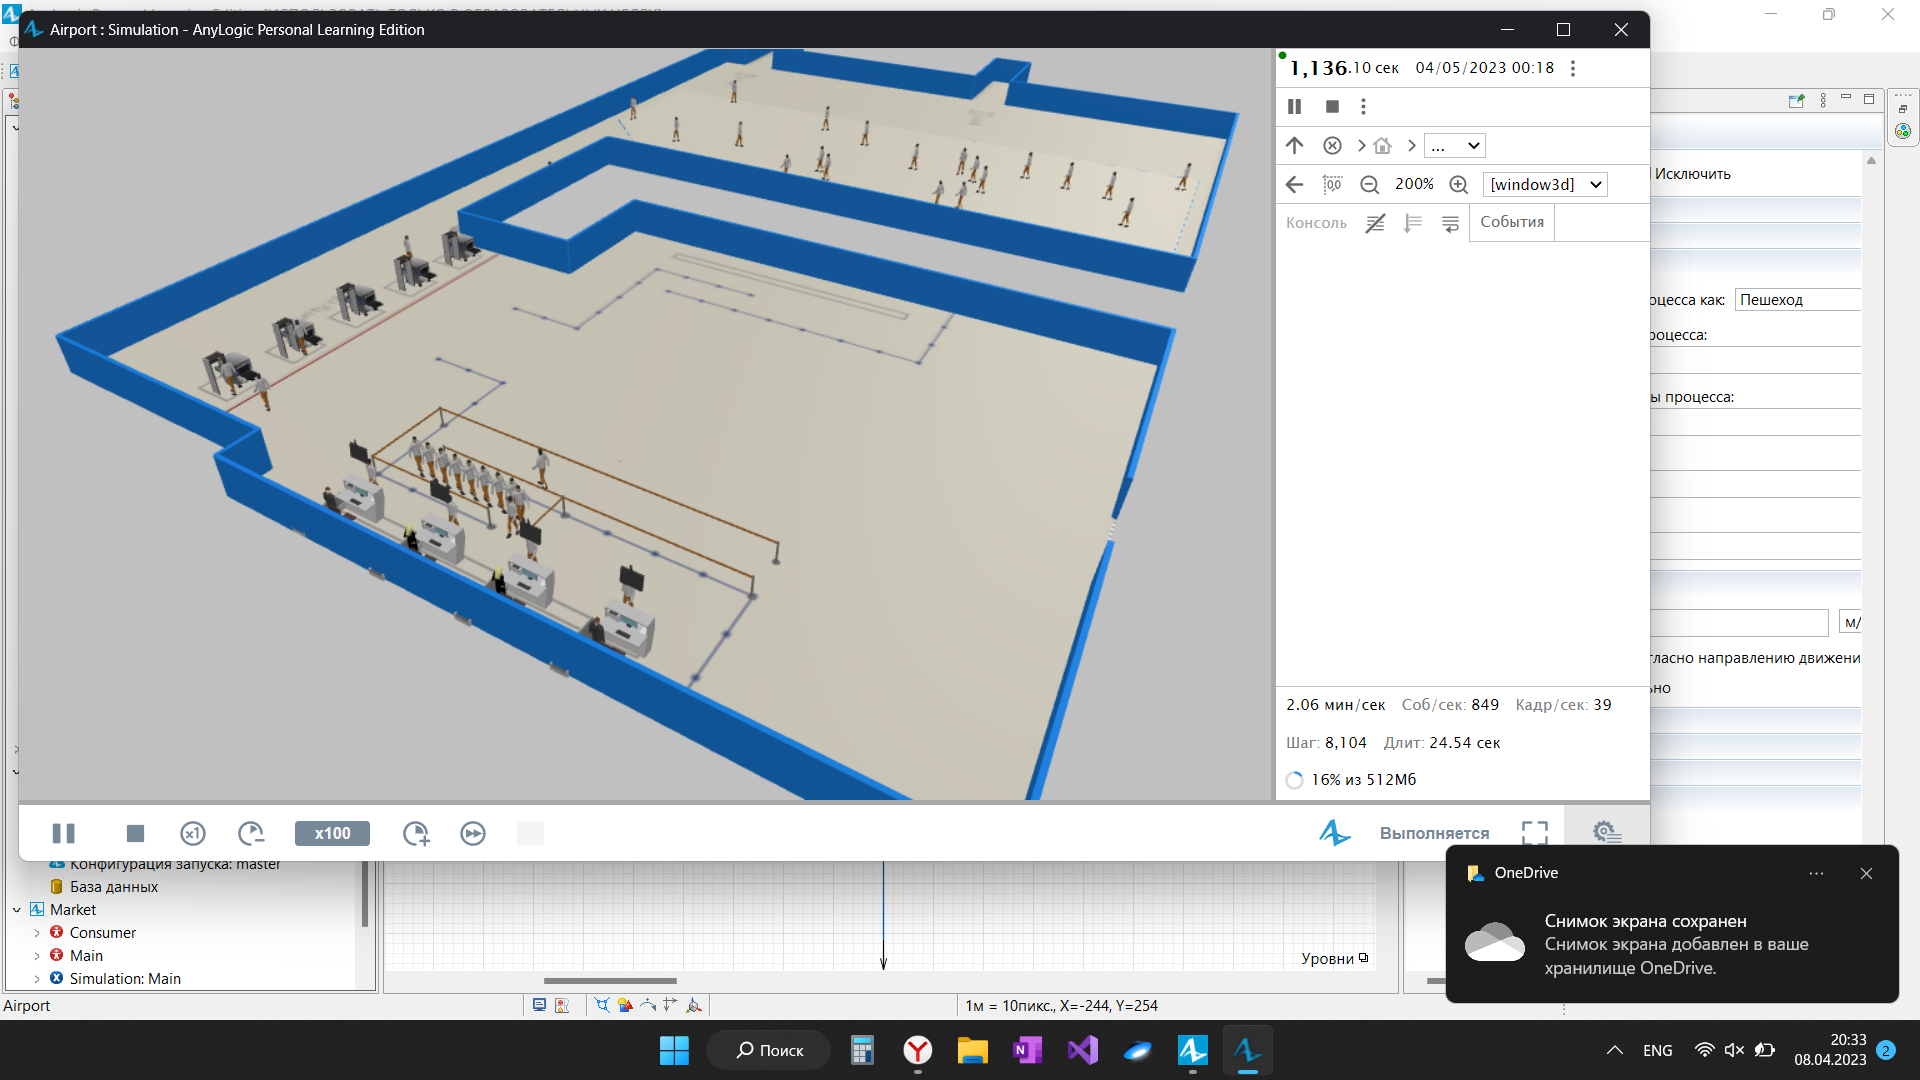
\includegraphics[width=0.9\textwidth]{2023-04-08 (1)}
	\caption{Простейшая дискретно-событийной модель}
	\label{fig:3d:anim}
\end{image}

\section{Моделирование предполетного досмотра пассажиров}
Теперь мы можем начать моделирование процессов, происходящих в
аэропорту.\par
Давайте начнем с моделирования процедуры предполетного досмотра
пассажиров. Для этого мы добавим в нашу модель пункты досмотра пассажиров.
С точки зрения терминологии пешеходного моделирования, пункт досмотра
является сервисом --- здесь пассажиры должны быть обслужены, а если пункт
досмотра в данный момент занят, то пассажирам приходится ждать в очереди,
пока он не освободится.\par
В моделируемом нами терминале находятся пять пунктов досмотра, поэтому
нам нужно будет добавить пять пунктов сервиса, к каждому из которых должна
вести очередь.\par
После того, как вы смените тип сервиса с точечного на линейный, точки
обслуживания сменят свою форму на линии.\par
Мы используем линейные сервисы, потому что хотим, чтобы пассажир следовал
вдоль линии сервиса и таким образом проходил через рамку металлодетектора,
как это и происходит при предполетном досмотре в аэропорту. Нам будет нужно
развернуть и переместить линии сервисов так, чтобы они пересекали
предполагаемые места расположения рамок металлодетекторов на плане
аэропорта.\par
Теперь, когда мы закончили рисование пунктов досмотра с помощью фигур
разметки пространства, мы можем добавить и сам процесс прохождения
предполетного досмотра в текущую логику модели. Для этого мы воспользуемся
специальным блоком Пешеходной библиотеки \texttt{PedService}, в свойствах
которого мы укажем наш элемент разметки пространства Сервис с очередями
\texttt{scpServices}.\par
Давайте добавим еще один блок диаграммы процесса, который будет
моделировать предполетный досмотр пассажиров.\par
Запустите модель. Вы увидите, что теперь пассажиры проходят процедуру
предполетного досмотра (Рисунок~\ref{fig:inspection}).

\begin{image}
	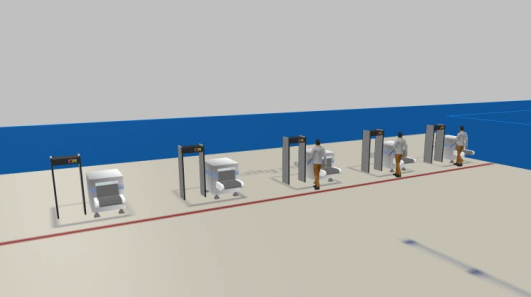
\includegraphics[width=0.9\textwidth]{Screenshot from 2023-04-11 14-57-23}
	\caption{Реализованная процедура досмотра}
	\label{fig:inspection}
\end{image}

\section{Добавление стоек регистрации}
Пассажиры могут регистрироваться на рейсы различными способами --- заранее
(онлайн-регистрация) или привычным образом --- в аэропорту у стоек
регистрации. Давайте добавим в нашу модель стойки регистрации на рейсы, и
направим туда тех пассажиров, кто не зарегистрировался на свой рейс
заблаговременно.\par
Переместите диаграмму процесса, собранную из блоков Пешеходной
библиотеки, выше оси X, вынеся ее тем самым за пределы области, видимой во
время работы модели. Если во время работы модели вам понадобится изучить
ход моделируемых процессов с помощью этой диаграммы, вы всегда можете
посмотреть на нее, просто переместив полотно окна модели с помощью мыши.\par
Поскольку пассажиры могут регистрироваться на рейсы различными способами,
нам нужно направить разные группы пассажиров в разные подпроцессы.\par
Мы хотим, чтобы прежде чем отправиться на посадку, пассажиры проводили
определенное время в зоне перед гейтами. Для этого нам нужно будет
нарисовать область ожидания, в которой пассажиры будут ожидать начала
посадки на рейс, а затем добавить в диаграмму процесса блок (PedWait),
который будет моделировать само ожидание.\par
Теперь запустив модель можно увидеть стойки регистрации и область ожидания
пассажиров перед посадкой (Рисунок~\ref{fig:registration}).

\begin{image}
	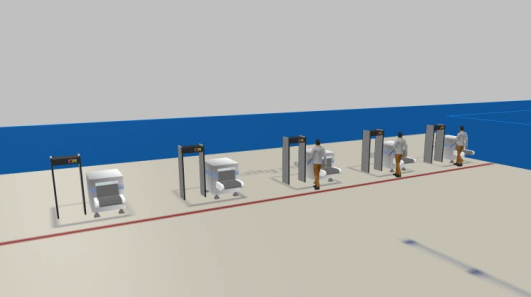
\includegraphics[width=0.9\textwidth]{Screenshot from 2023-04-11 14-57-23}
	\caption{Реализованная процедура регистрации}
	\label{fig:registration}
\end{image}

\section{Моделирование посадки на самолет}
Пассажиры будут ожидать начала посадки на рейс в области ожидания (общей
для обоих выходов на посадку). Когда начнется посадка, они должны будут
пройти процедуру проверки посадочных талонов, после чего они смогут пройти
на борт самолета.\par
К стойке проверки посадочных талонов и документов ведут две очереди – одна
для пассажиров бизнес-класса, другая – для пассажиров эконом-класса.
Проверка документов каждого пассажира занимает в среднем от 1 до 3 секунд.\par
Нам нужно как-то отличать в нашей модели пассажиров бизнес-класса от
пассажиров эконом-класса. Для этого потребуется хранить дополнительную
информацию о пассажире в заданном нами ранее типе пешехода.\par
Мы хотим, чтобы пассажиров, летящих разными классами, можно было легко
различить визуально на анимации модели. Для этого мы будем использовать
две разные 3D модели людей для отображения пассажиров бизнес-класса и
эконом-класса.\par
Мы будем задавать класс пассажира в момент его создания блоком PedSource.\par
Запустите модель. Вы увидите, как служащие аэропорта проверяют
посадочные талоны пассажиров. Пассажиры встают в одну из двух очередей
в зависимости от того, имеют ли они право на приоритетное обслуживание
или нет (Рисунок~\ref{fig:landing}).

\begin{image}
	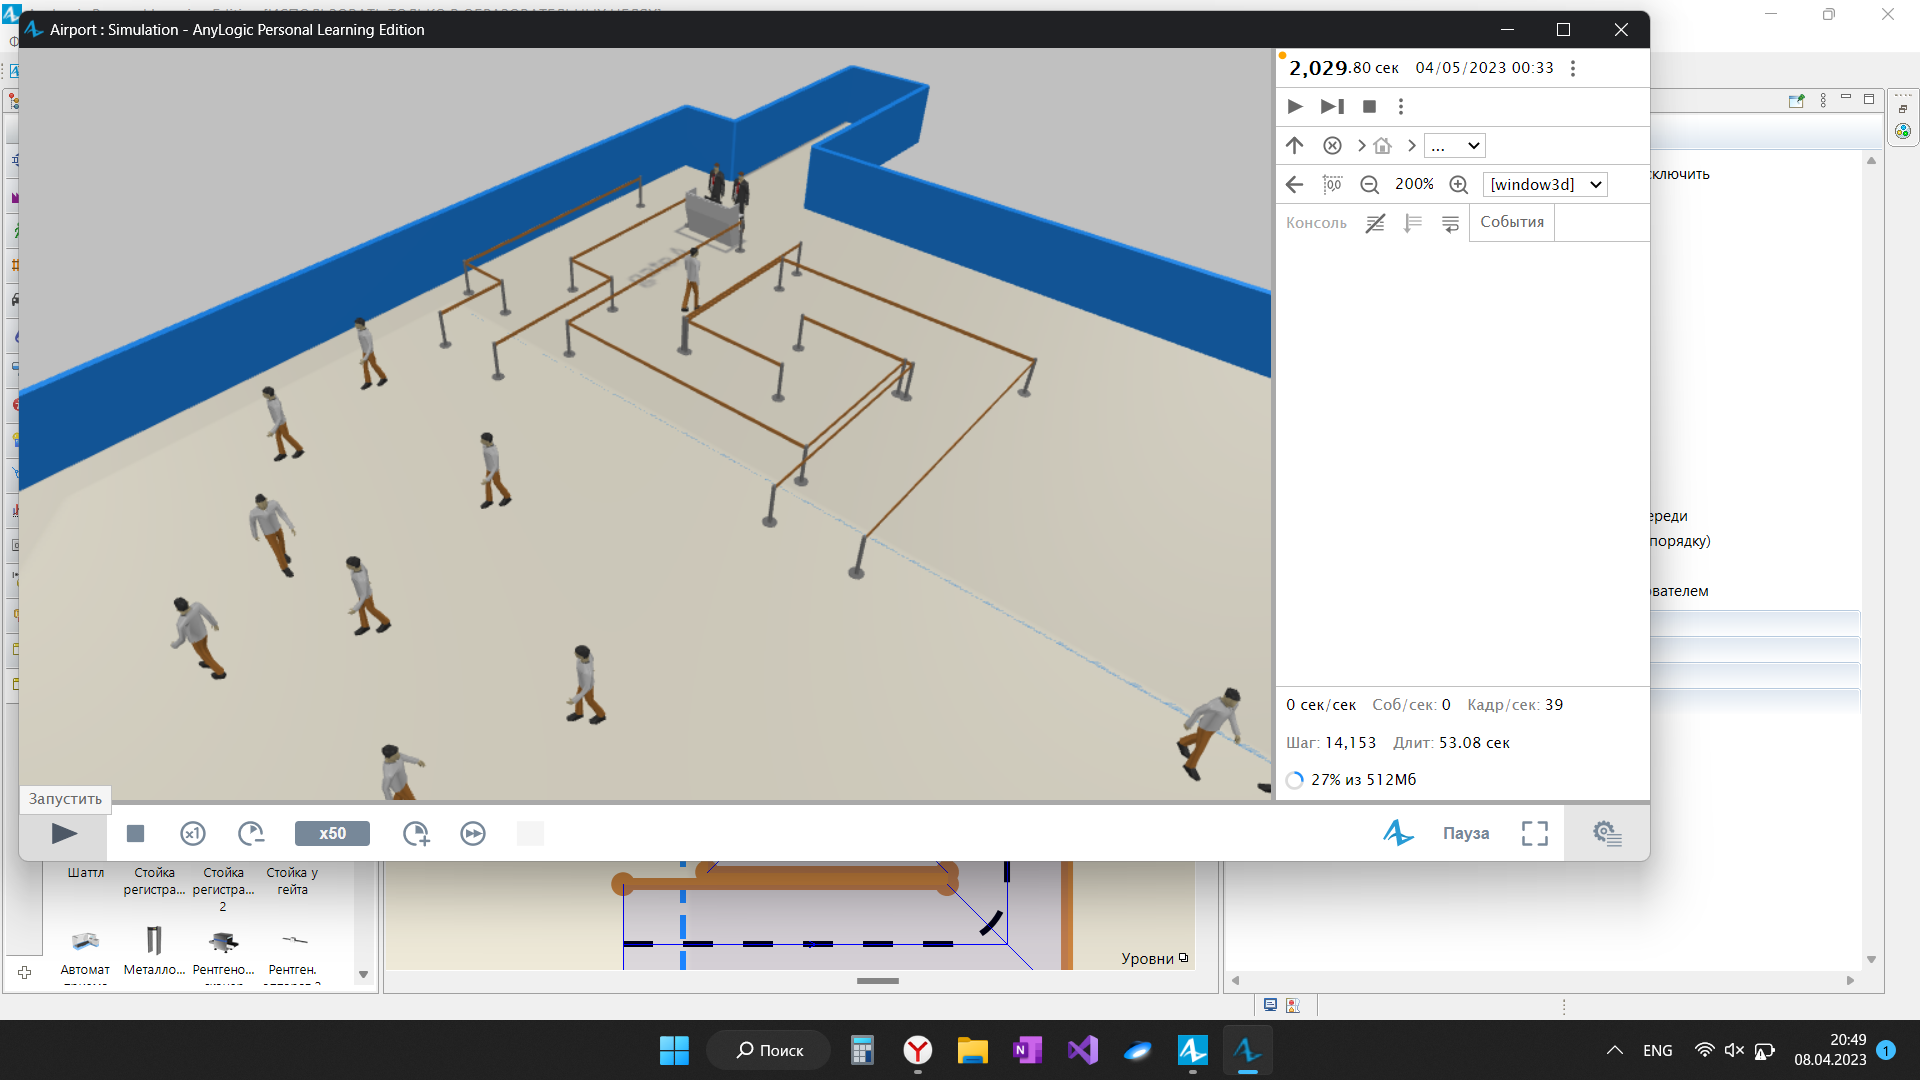
\includegraphics[width=0.9\textwidth]{2023-04-08 (2)}
	\caption{Посадка пассажиров}
	\label{fig:landing}
\end{image}

\section{Считывание данных о рейсах из файла MS Excel}
Теперь мы добавим в нашу модель рейсы, считав расписание вылетов из
таблицы Excel.
В каждой модели AnyLogic есть своя встроенная база данных, в которой могут
храниться значения входных параметров модели, а также результаты работы
модели.
База данных AnyLogic позволяет:

\begin{itemize}
	\item Конфигурировать модель согласно заданным в БД параметрам.
	\item Параметризовать популяции агентов.
	\item Задавать частоту прибытия агентов-заявок в процессных моделях.
	\item Импортировать данные из других БД или таблиц Excel и хранить их в
		доступной форме.
	\item Записывать логи (журналы выполнения) модели, в которые добавляется
		информация обо всех произошедших событиях в диаграммах
		процессов, диаграммах состояний, статистика по взаимодействию и
		перемещению агентов, и т.д.
	\item Сохранять и экспортировать статистику, хранящуюся в наборах данных.
	\item Экспортировать данные в электронные таблицы MS Excel.
	\item Создавать резервные копии БД.
\end{itemize}

Мы покажем, как импортировать данные из внешней базы данных во
встроенную БД модели.
Запустите модель. Вы увидите, как пассажиры ожидают объявления о
начале посадки на рейс, после чего направляются к гейту для прохождения
процедуры проверки посадочных талонов (Рисунок~\ref{fig:excel}).

\begin{image}
	%\includegraphics[width=0.9\textwidth]{}
	\caption{Использование базы данных}
	\label{fig:excel}
\end{image}


\clearpage

\section*{\LARGE Вывод}
\addcontentsline{toc}{section}{Вывод}
В данной практической работе была создана простая модель аэропорта
основанная на пешеходном моделировании, описывающая процессы
от входа пассажирова в аэропорт до их посадки в самолет
Теперь мы обладаем базовыми знаниями о создании потоков
пешеходов, создании 3D анимации и считывании данных о рейсах из файла Excel.

